\documentclass{standalone}
\usepackage[standard-baselineskips]{cmbright}
\renewcommand\familydefault{\sfdefault}
\usepackage[T1]{fontenc}

\usepackage{amsmath,amssymb,latexsym,float,epsfig,hyperref}
\usepackage{framed,color,url,fancybox,fullpage,booktabs,subfigure,wrapfig,chngpage,setspace}
\usepackage[latin1]{inputenc}
\usepackage{tikz}

\usetikzlibrary{shapes,arrows}
\usetikzlibrary{arrows,positioning,mindmap} 
\usetikzlibrary{calc,trees,positioning,arrows,chains,shapes.geometric,%
decorations.pathreplacing,decorations.pathmorphing,shapes,%
matrix,shapes.symbols,plotmarks,decorations.markings,shadows}
\usetikzlibrary{patterns}

\tikzstyle{decision} = [diamond, draw, fill=gray!10,
  text width=6em, text badly centered, node distance=2.5cm, 
  inner sep=0pt,minimum height=1em,text centered]
\tikzstyle{block} = [rectangle, draw, fill=blue!20,
  text width=10em, text centered, rounded corners, minimum height=3.0em]
\tikzstyle{cloud} = [draw, ellipse,fill={rgb:orange,1;yellow,1;pink,1}, node distance=4cm,
    minimum height=1em,text centered]
\tikzstyle{circ} = [draw,circle,fill={rgb:orange,1;yellow,1;pink,1}, 
  node distance=4cm, minimum height=2em, text centered]

\tikzstyle{line} = [draw, very thick, color=black, -latex']
\tikzstyle{redline} = [draw, very thick, color=red, -latex']
\tikzstyle{dotline} = [draw,dotted, very thick, color=black!50, -latex']

% % % \include{tableau_colors} in your .tex file to use these custom
% Tableau colors
% https://gist.github.com/AndiH/c957b4d769e628f506bd

\definecolor{dblue}{RGB}{31, 119, 180}
\definecolor{lblue}{RGB}{174, 199, 232}

\definecolor{dorange}{RGB}{255, 127, 14}
\definecolor{lorange}{RGB}{255, 187, 120}

\definecolor{dgreen}{RGB}{44, 160, 44}
\definecolor{lgreen}{RGB}{152, 223, 138}

\definecolor{dred}{RGB}{214, 39, 40}
\definecolor{lred}{RGB}{255, 152, 150}

\definecolor{dpurple}{RGB}{148, 103, 189} 
\definecolor{lpurple}{RGB}{197, 176, 213}

\definecolor{dbrown}{RGB}{140, 86, 75} 
\definecolor{lbrown}{RGB}{196, 156, 148}    

\definecolor{dpink}{RGB}{227, 119, 194}
\definecolor{lpink}{RGB}{247, 182, 210}

\definecolor{dgray}{RGB}{127, 127, 127}
\definecolor{lgray}{RGB}{199, 199, 199}

\definecolor{dolive}{RGB}{188, 189, 34}
\definecolor{lolive}{RGB}{219, 219, 141}

\definecolor{dskyblue}{RGB}{23, 190, 207}
\definecolor{lskyblue}{RGB}{158, 218, 229}

\definecolor{gold}{RGB}{255,223,0}
 in your .tex file to use these custom
% Tableau colors
% https://gist.github.com/AndiH/c957b4d769e628f506bd

\definecolor{dblue}{RGB}{31, 119, 180}
\definecolor{lblue}{RGB}{174, 199, 232}

\definecolor{dorange}{RGB}{255, 127, 14}
\definecolor{lorange}{RGB}{255, 187, 120}

\definecolor{dgreen}{RGB}{44, 160, 44}
\definecolor{lgreen}{RGB}{152, 223, 138}

\definecolor{dred}{RGB}{214, 39, 40}
\definecolor{lred}{RGB}{255, 152, 150}

\definecolor{dpurple}{RGB}{148, 103, 189} 
\definecolor{lpurple}{RGB}{197, 176, 213}

\definecolor{dbrown}{RGB}{140, 86, 75} 
\definecolor{lbrown}{RGB}{196, 156, 148}    

\definecolor{dpink}{RGB}{227, 119, 194}
\definecolor{lpink}{RGB}{247, 182, 210}

\definecolor{dgray}{RGB}{127, 127, 127}
\definecolor{lgray}{RGB}{199, 199, 199}

\definecolor{dolive}{RGB}{188, 189, 34}
\definecolor{lolive}{RGB}{219, 219, 141}

\definecolor{dskyblue}{RGB}{23, 190, 207}
\definecolor{lskyblue}{RGB}{158, 218, 229}

\definecolor{gold}{RGB}{255,223,0}
 in your .tex file to use these custom
% Tableau colors
% https://gist.github.com/AndiH/c957b4d769e628f506bd

\definecolor{dblue}{RGB}{31, 119, 180}
\definecolor{lblue}{RGB}{174, 199, 232}

\definecolor{dorange}{RGB}{255, 127, 14}
\definecolor{lorange}{RGB}{255, 187, 120}

\definecolor{dgreen}{RGB}{44, 160, 44}
\definecolor{lgreen}{RGB}{152, 223, 138}

\definecolor{dred}{RGB}{214, 39, 40}
\definecolor{lred}{RGB}{255, 152, 150}

\definecolor{dpurple}{RGB}{148, 103, 189} 
\definecolor{lpurple}{RGB}{197, 176, 213}

\definecolor{dbrown}{RGB}{140, 86, 75} 
\definecolor{lbrown}{RGB}{196, 156, 148}    

\definecolor{dpink}{RGB}{227, 119, 194}
\definecolor{lpink}{RGB}{247, 182, 210}

\definecolor{dgray}{RGB}{127, 127, 127}
\definecolor{lgray}{RGB}{199, 199, 199}

\definecolor{dolive}{RGB}{188, 189, 34}
\definecolor{lolive}{RGB}{219, 219, 141}

\definecolor{dskyblue}{RGB}{23, 190, 207}
\definecolor{lskyblue}{RGB}{158, 218, 229}

\definecolor{gold}{RGB}{255,223,0}


\begin{document}

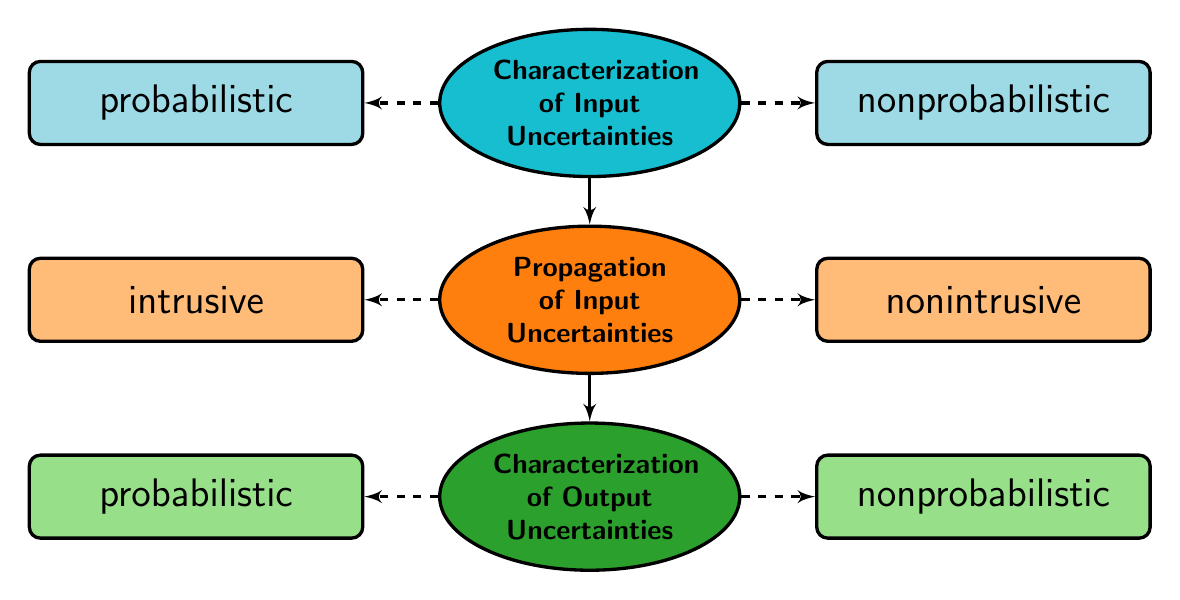
\begin{tikzpicture}[auto]
  \def\dy{2.5};
  \node [cloud, very thick, node distance=3.5cm, text width=7em, fill=dskyblue,font=\bfseries] (1) at (0,0) {{Characterization of Input Uncertainties}};
  \node [block, very thick, node distance=5.0cm, inner ysep=0em, text width=4cm,fill=lskyblue,font=\Large] (1A)  at  (5,0) {
    nonprobabilistic
  };  
  \path [line, dashed] (1) -- (1A);
  \node [block, very thick, node distance=5cm, inner ysep=0em, text width=4cm,fill=lskyblue,font=\Large] (1a) at (-5,0) {
    probabilistic
  };  
  \path [line, dashed] (1) -- (1a);

  \node [cloud, very thick, node distance=3.5cm, text width=7em, fill=dorange, font=\bfseries] (2) at (0,-\dy) {{Propagation of Input Uncertainties}};
  \node [block, very thick, node distance=5cm, inner ysep=0em, text width=4cm,fill=lorange,font=\Large] (2A)  at  (5,-\dy) {
    nonintrusive
  };  
  \path [line, dashed] (2) -- (2A);
  \node [block, very thick, node distance=5cm, inner ysep=0em, text width=4cm,fill=lorange,font=\Large] (2a) at (-5,-\dy) {
    intrusive
  };  
  \path [line, dashed] (2) -- (2a);
  \path [line, very thick] (1) -- (2);

  \node [cloud, very thick, node distance=3.5cm, text width=7em, fill = dgreen, font=\bfseries] (3) at (0,-2*\dy) {{Characterization of Output Uncertainties}};
  \node [block, very thick, node distance=5cm, inner ysep=0em, text width=4cm, fill=lgreen,font=\Large] (3A)  at  (5,-2*\dy) {
    nonprobabilistic
  };  
  \path [line, dashed] (3) -- (3A);
  \node [block, very thick, node distance=5cm, inner ysep=0em, text width=4cm, fill=lgreen,font=\Large] (3a) at (-5,-2*\dy) {
    probabilistic
  };  
  \path [line, dashed] (3) -- (3a);
  \path [line] (2) -- (3);
\end{tikzpicture}

\end{document}
